\chapter{Introduction}
%% Proposed roadmap
%
%   The use of RT in the industrial environments
%   Current standards IEEE and IEC and the TSN
%           Roadmap of standards
%           RTE protocols and OPC UA   
%           How are they related
%  
%   -----------State of the art--------------------------------
%   Applications with RTE and OPC UA in Hard Real Time applications     
%   A brief overview about the RT tools in robotics
%           The importance of EtherCAT as an open RTE protocol within robotics
%   Comparison of openess
%   EtherCAT introduction (selected by Hans Robot)
%           Focus on EtherCAT XoE <<THIS ONLY NEEDS TO BE MENTIONED
%------------------Out of scope--------------------------------------
%   HW ASICS and stuff like that
%   SW Stacks for EtherCAT development and other RTEs
%
%

% Terms:
% ACB = Axis communication board, alias for embedded communication hub for sensor data acquisition in a robotic system
% RTE = Real-Time Ethernet as specified in IEC 61784-2:2019. \cite{rte:standards}
% IIoT = Industrial Internet of Things

% 100/100
This document describes the different stages through the development of an embedded communication hub for sensor
data acquisition in a robotic system, that will be the starting point of a framework for the development of 
devices used within an industrial robot. In this document the prototype will be referred as \emph{Axis Communication Hub} or ACB. 

During this first chapter a brief introduction to the Real-Time Ethernet (RTE) industrial networks is presented, as well as 
a summary of the standards involved with comments about how they are related to each other. 
The second chapter shows a summary of the state of the art regarding the possibilities for developing open source projects 
according to the degree of openness of an RTE communication protocol. Moreover, the usage of these RTE 
industrial protocols in embedded applications and its relation to the Industrial Internet of Things (IIoT) necessities is 
briefly introduced. At the end of this chapter, a brief comparison of the openness of these protocols and how this is related 
to the development of devices is presented.  The applications introduced have to do mainly with EtherCAT, as it is within 
the scope of this Research Project, showing advantages that will be detailed as the reader reads through this document. 
Afterwards, the third chapter deals with the technical specification of this Research Project and its development proposal, 
including the hardware available, firmware structure and the overall prioritization of the goals. 
Later on, during the fourth chapter, the main points related to the implementation process are presented. 
In chapter five the overall results are discussed, where the reader can find comments about the implementation and test 
challenges and their solutions. In the sixth chapter the conclusions are summarized. 
Finally, extra information focused on the technical details of the project, such as diagrams or protocol-related specifications, 
can be found within the appendixes.

\section{The need of RT within industrial environments}

During the last years an increase in the usage of the Ethernet-based field buses within industry has been recorded. This
shows the expected adaptation of the industrial automation to the IT infrastructure, which is fundamental for the \emph{Industry 4.0} paradigm
and its consequent huge amount of data to be monitored, analyzed and controlled. This data deals at the same time with different time constraints 
and interconnectivity among the different layers of an industrial system and all their devices. 
Having in mind that the former \emph{automation pyramid}, see in Fig.~\ref{fig:pyramid-classic}, where the different layers needed various gateways
to communicate in a rather vertical approach, has been evolving to a one more flexible structure; it is then understandable 
that several technologies providing this access have been meeting each other while coming either from the top or the down levels. A good 
overview of the mentioned structures can be read in \cite{tsn_intro}.
Nowadays, these technologies offer similar features regarding data access and security, each of them with their own development 
history, alliances and, therefore, standards. 
\begin{figure}[h]
    \centering
    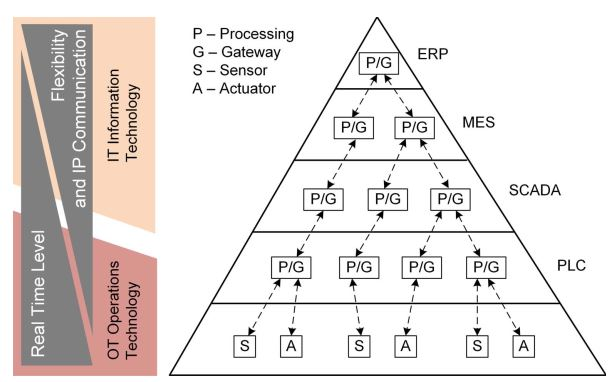
\includegraphics[width=0.7\textwidth]{imgs/intro-industryarchitecture2.jpg}
    \caption{Classical automation pyramid structure, source from \cite{tsn_intro}.}
    \label{fig:pyramid-classic}
\end{figure}

Coming from top-level-related frameworks, there is, e.g., the OPC UA project; whereas names like Profinet,
DeviceNET, EtherCAT, Powerlink, etc, come from the field bus side---the lowest level. All of them have developed in an individual way as response
to market needs, however meeting in the late decade through the necessity for unified standards to improve interoperability between the incredible number
of projects. This happens at a time were information, technical as well, and development tools have become even more available and
open to the end-user and the developer. Leading then now to a situation where the private initiatives are not any longer the full owners of the technology development.
See Fig.~\ref{fig:pyramid-iiot} for the IIoT's approach.

\begin{figure}[h]
    \centering
    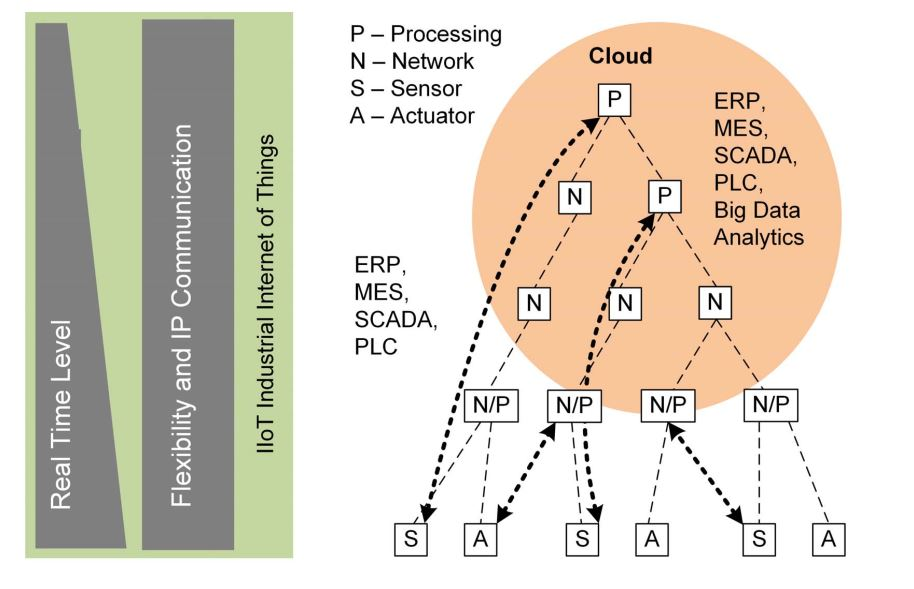
\includegraphics[width=0.7\textwidth]{imgs/intro-industryarchitecture.jpg}
    \caption{\emph{Industry 4.0} a more flexible automation structure. Industrial Internet of Things, source from \cite{tsn_intro}.}
    \label{fig:pyramid-iiot}
\end{figure}

Another line of work, closely related to interoperability, is the Real Time (RT) applications in their both versions with \emph{hard} and \emph{soft} requirements. 
Nowadays, there is an increasing number of applications in robotics that demand control loops and device chains that
require hard real time performance. Although these requirements are more common at the operational technology level, such as, robots, CNCs, servo motors, etc. 
They all face now the IIoT demands; hence, their networks should meet as well certain degree of RT capability. 
Moreover, synchronization of time sensitive
systems within manufacturing lines, for instance, has been addressed for years by the RTE protocols and now this kind of features are increasingly
been demanded as well at upper layers.

The current automation industry has a record of many competitors and close technologies, as natural consequence for specific processes requirements (depending on the industry), 
but also as a response of market strategies. Nevertheless, the search for standardization
can be tracked back to the \SI{80}{\second}, as the field buses were standardized by the International Electrotechnical Commission (IEC). 
Continuing doing so until the Ethernet took its place within the industry. As an important note, during the last two years, according to the HMS Industrial Networks' annual study,
the total market shares of new industrial nodes in factory automation increased for the Industrial Ethernet from \num{52}$\%$ to \num{64}$\%$; while the commonly called
field buses decreased in the same period from $42\%$ to only $30\%$. Finally, the industrial wireless remained around the \num{6}$\%$, see Fig.\ref{fig:fieldbus_shares}.

It is yet worthy to mention that the name \emph{Industrial Ethernet} is used only as a 
generalization for the group of protocols that historically developed on IEEE's Ethernet specification; even though they all are almost no further
compatible with each other---as they have modified Media Access Control (MAC) Layers. More details about these differences will be addressed in the following chapters.  

\begin{figure}[h]
    \centering
    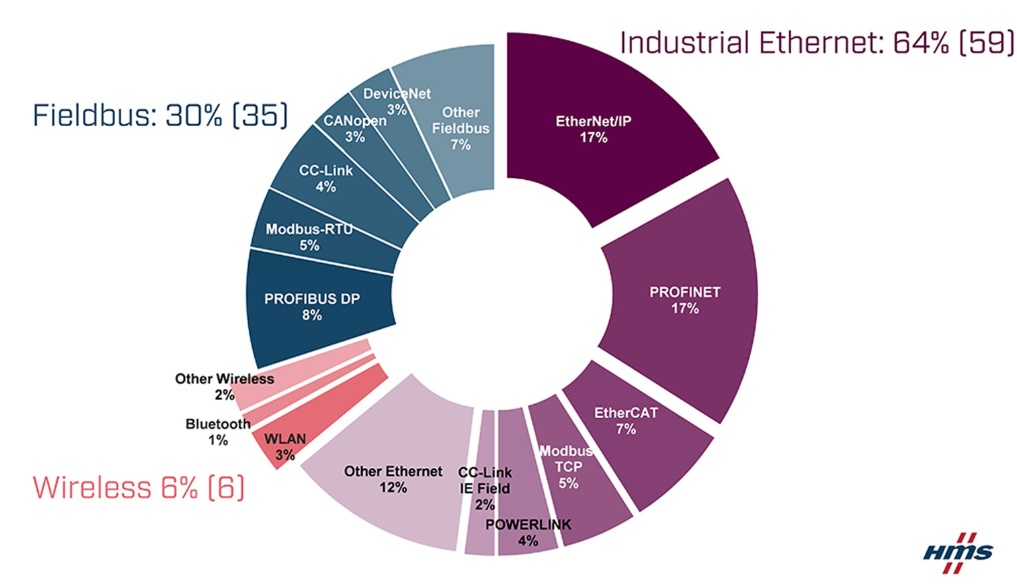
\includegraphics[width=.8\textwidth]{imgs/intro-buses-share.jpg}
    \caption{Industrial network market shares 2020 according to HMS Networks. Source from \cite{fieldbus_shares}.} %Add the reference, this could be a table
    \label{fig:fieldbus_shares}
\end{figure}

Vendor protected technology has its limit when there are plenty of possibilities for automation technologies, even if they are in ongoing development. 
For instance, as happened during the lifetime of the Open Platform Communications (OPC) project---predecessor of OPC UA---that was started only upon Microsoft Windows and 
as the time went by, the emerging needs made it change to use open standards and a multiplatform approach.

To introduce the reader to a common ground regarding standardization, the following section will present a brief summary of the standards that 
are of interest for anyone who wants to start developing using industrial interfaces.

\section{Industrial standards and the TSN initiative}\label{sec:standards} 

This section is intended to provide the starting developer a rough but useful reference of the standards related to industrial 
communication networks. 

First, due to the historical and technological process of innovation within the information and communication 
systems, several parties have been related and, at some extension have merged results, bringing out an interconnected 
set of norms that thrive continuously onto a global standardization.

The following list is intended to be a quick reference to the current standards for Ethernet, legacy and current field buses, 
Time-Sensitive Networks in their American and international initiatives. This way, the reader has a roadmap to be taken into
account for deeper research within the industrial applications. 
Furthermore, information related to the similar standardization processes between 
the IEC, ISO and IEEE, and their unavoidable cooperation, can be read in \cite{standards_coop}. %a comparisson of the ieee and iec standars processes

\begin{description}
    \item[ISO/IEC/IEEE 8802-3:2015] Revision of the Ethernet standard for half and full-duplex communication up to \SI{100}{\mega\bit\per\second}. 
    Originally published by American IEEE 802-3 in 1985 and accepted internationally in 1989. The last revision 8802-3-2017/Amd 10-2019 includes
        MAC controls for \SIlist{200;400}{\giga\bit\per\second}. More information in \cite{iso8802_ethernet}. %https://www.iso.org/standard/72048.html 
        After 2019 The name Ethernet is not longer used, instead CSMA/CD or a reference to the corresponding ISO standard 8802.3 is the formal name.
    \item[IEC 61158:1999-2000] First international field bus standard published in 1999, where 8 \emph{Types} of field buses were introduced addressing the 
        Physical Layer (PhL), the services and protocols of Data Link Layer (DLL) and Application Layer (AL). Some included brand 
        names were the following: H1/HSE/H2, ControlNet, EtherNET/IP, Profibus, Profinet, Interbus. This standard has an interesting story
        concluding with the signing of the \emph{Memorandum of Understanding} by the main contenders to put end to the field bus war. The latter can be reviewed in \cite{fieldbus_history}.%The Fieldbus Standards: History and Structures
         The standard's most updated version in 2019 includes 26 Types of protocols, creating out of them the so-called Communication Profiles (CP), likewise grouped
        into field bus Communication Profile Families (CPF). 
    \item[IEC 61784-Part 2:2008] It is extension for the RT capable CPs that are based on the IEEE 8802-3 standard. Commercial names included 
        are the next: EtherCAT, Profinet, Ethernet/IP, Ethernet Powerlink, and Modbus TCP. An interesting overview of the current development 
        of the industrial communication networks can be reviewed in \cite{future_iiot}. %Industrial Communication Systems and Their Future Challenges: Next-Generation Ethernet, IIoT, and 5G
        The SERCOS CPF is highlighted, since its third version is, altogether with the EtherCAT profile, the fastest one in the list; providing as well
        a more efficient use of the available bandwidth with an open source resources. It shows even advantages over CAN devices due
        to its original design intended for hard RT motion control; for more information review \cite{sercos_origin} and \cite{sercos_performance}. %https://www.designnews.com/sercos-picks-pace %https://www.sercos.org/technology/advantages-of-sercos/performance/. 
        This is a very interesting hard RT protocol whose applications might need further study out of the scope of this 
        Research Project.
    \item[IEEE 802.1A/B/C/D/Q] Time-Sensitive Networking standards is an initiative to improve the IEEE 802-3 in order to meet the industrial real time requirements, 
        which story can be tracked back to 2005, as the IEEE 802-3 group was merged with the IEEE 802.1 Audio Video Bridging Task Group and started to work for
        industrial environments. This a response to the vast alternatives of the RTE CPs. About 60 individual IEEE standards oriented to improve
        the ISO/OSI layer 2, including 13 focused on its security, are within the scope of the TSN project. A nice introduction to this standard's scope can be read from TSN 
        section in \cite{future_iiot}. %section about the TSN
        The mentioned project covers the lower layers of the communication system, whereas the upper ones, representation and transfer of data, is
        addressed by OPC UA. Moreover, it is important to mention that this is an ongoing project and still around $40\%$ of its standards are
        in draft or preparation phase. For further information regarding the current standard development, visit \cite{tsn_homepage}.
    \item[IEC/IEEE 60802] TSN Profile for Industrial Automation is the stand alone TSN base standard that will include the common advancements
        from IEC SC65C/WG18 and IEEE 802 work groups mentioned in the previous item. See \cite{tsn_profile} for the current development group's activities. %https://1.ieee802.org/tsn/iec-ieee-60802/
        This is an ongoing project started around 2017, still being in a draft phase. Since this will be the international standard, it would be 
        the equivalent to the effort once given during the creation of the IEC 61158 for the legacy field buses.
    \item[IEC 62541:2016-2020] Set of IEC standards for OPC UA. Individually, the IEC 62541-14:2020 defines the OPC Unified Architecture 
        (OPC UA) PubSub communication model. It defines an OPC UA publish/subscribe pattern which complements the client server pattern defined 
        by the Services in IEC 62541-4. IEC TR 62541-1 gives an overview of the two models and their distinct uses. For the concrete list of contents, review \cite{opcua_standard}. %https://webstore.iec.ch/publication/61108  
        An overview of this technology and how it is planned to complement the TSN can be reviewed in \cite{opc_tsn_application}. %Open Source OPC UA PubSub over TSN for Realtime Industrial Communication
\end{description}



% CANopen protocol is not capable of hard real time capabilities?


% >>Here comes information about SERCOS. The SERCOS interface started as a project for providing a Hard Real Time capable communication
% bus, it has been developed during the years, having nowadays three versions. The first ones operating over a serial bus and submitted
% to the IEC, which in 1995 released it as IEC 61491.[2] After the release of the original standard, original working group member companies 
% including ABB, AEG, AMK, Robert Bosch, Indramat, and Siemens founded the "Interest Group Sercos" to steward the standard. \ref{dummy} %https://en.wikipedia.org/wiki/SERCOS_interface#cite_note-3
% Even though the capabilities meet hard real time requirments, compared to other technologies, is rather limited. %https://en.wikipedia.org/wiki/SERCOS_interface#cite_note-3
% For the last version it has been capable to address up to 60 Motion Axes and makes use of the Ethernet standard, making it an alternative
% for the mentioned technology comming from BEckhoff. Together with EtherCAT, Sercos is the fastest 100Mps industrial Ethernet technology.
% One advantage so far of this protocol is its parallel development with the OPC UA, making it natively compatible with such networks* 
% and security layers.


